\documentclass{standalone}
\usepackage{tikz}
\usepackage{pgfplots}
\pgfplotsset{compat=1.18}

\begin{document}
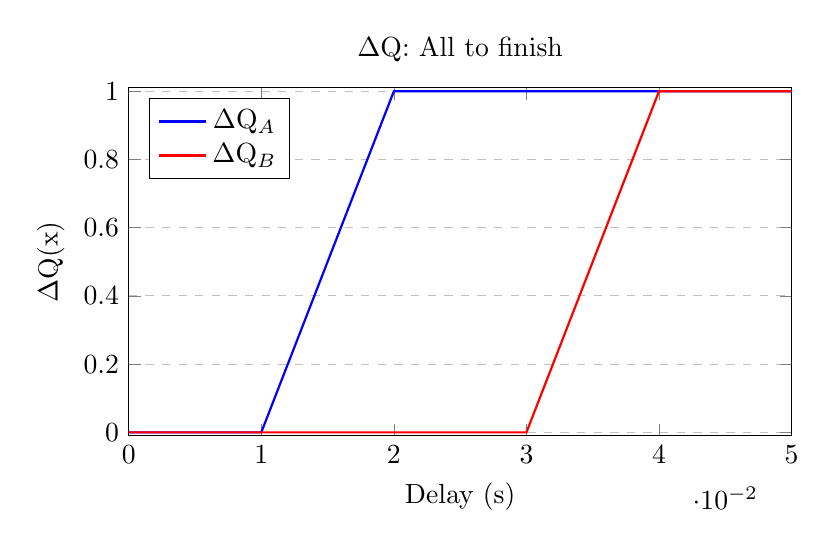
\begin{tikzpicture}
\begin{axis}[
    title={$\Delta$Q: All to finish},
    xlabel={Delay (s)},
    ylabel={$\Delta$Q(x)},
    xmin=0, xmax=0.05,
    ymin=-0.01, ymax=1.01,
    xtick={0, 0.01, 0.02, 0.03, 0.04, 0.05},
    ytick={0,0.2,0.4,0.6,0.8,1},
    ymajorgrids=true,
    grid style=dashed,
    width=10cm,
    height=6cm,
    legend pos = north west,
]
\addplot[color=blue, mark=none, thick] coordinates {
    (0.00, 0.00)
    (0.01, 0.00)
    (0.02, 1)
    (0.05, 1)
};
\addlegendentry{$\Delta$Q$_A$}

\addplot[color=red, mark=none, thick] coordinates {
    (0.00, 0.00)
    (0.03, 0.00)
    (0.04, 1)
    (0.05, 1)
};
\addlegendentry{$\Delta$Q$_B$}
\end{axis}
\end{tikzpicture}
\end{document}
